\begin{figure}[h]
    \centering{
    \begin{tabular}{ccc}
        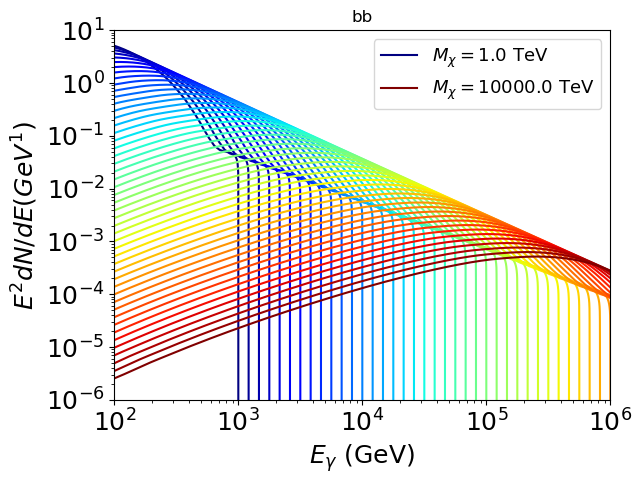
\includegraphics[scale=0.27]{figures/mtd_hawc_dm/hdm_bb.png} &
        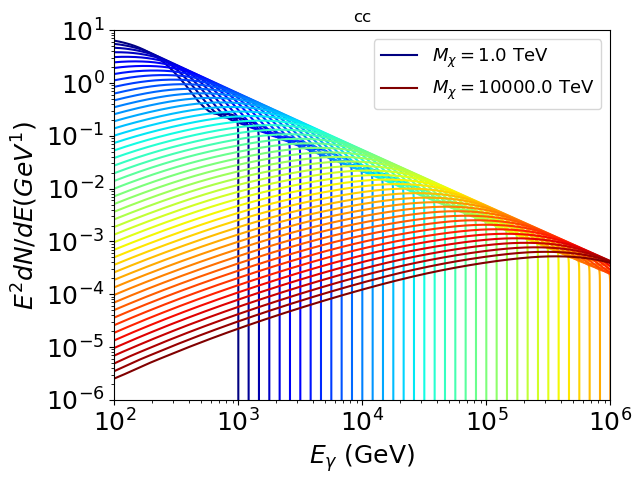
\includegraphics[scale=0.27]{figures/mtd_hawc_dm/hdm_cc.png} &
        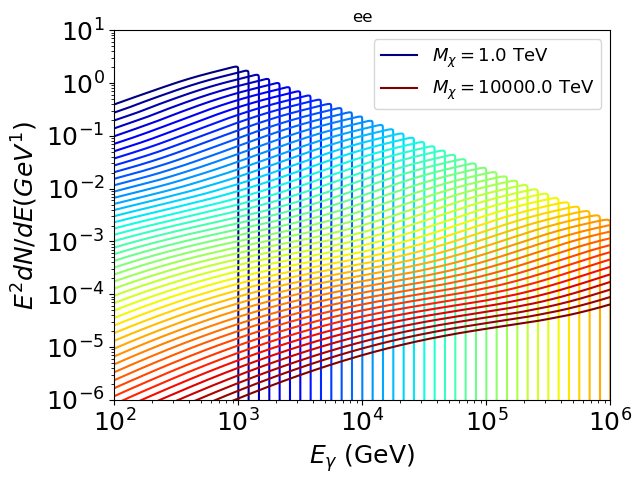
\includegraphics[scale=0.27]{figures/mtd_hawc_dm/hdm_ee.png} \\
        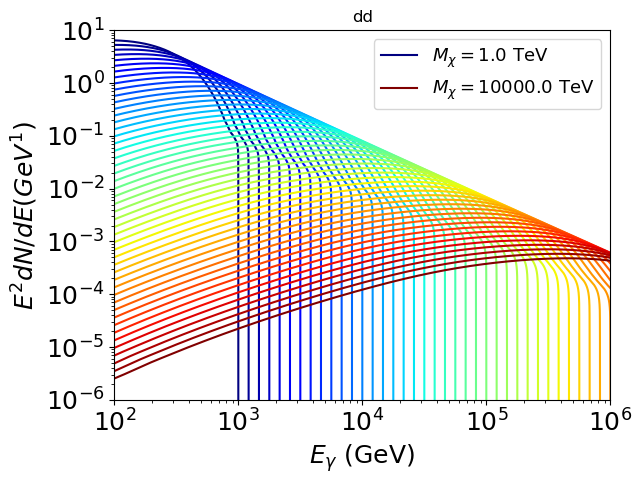
\includegraphics[scale=0.27]{figures/mtd_hawc_dm/hdm_dd.png} &
        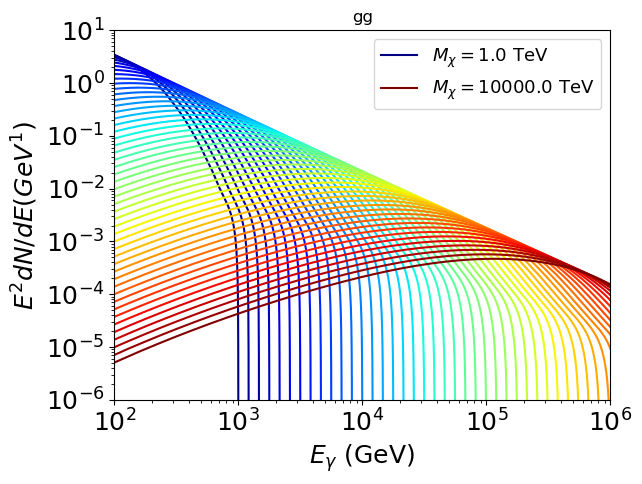
\includegraphics[scale=0.27]{figures/mtd_hawc_dm/hdm_gg.png} &
        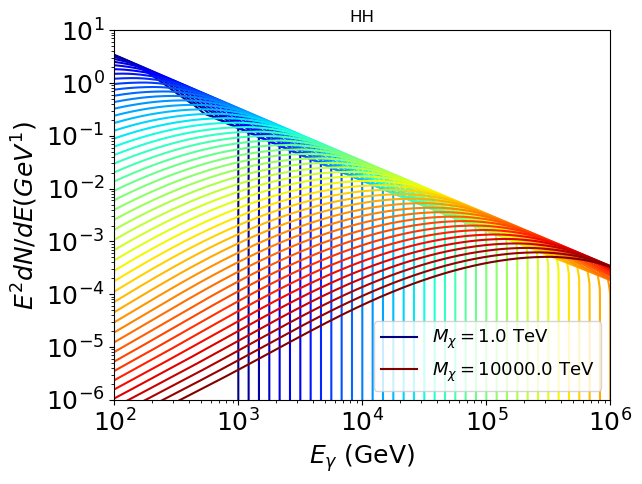
\includegraphics[scale=0.27]{figures/mtd_hawc_dm/hdm_hh.png} \\
        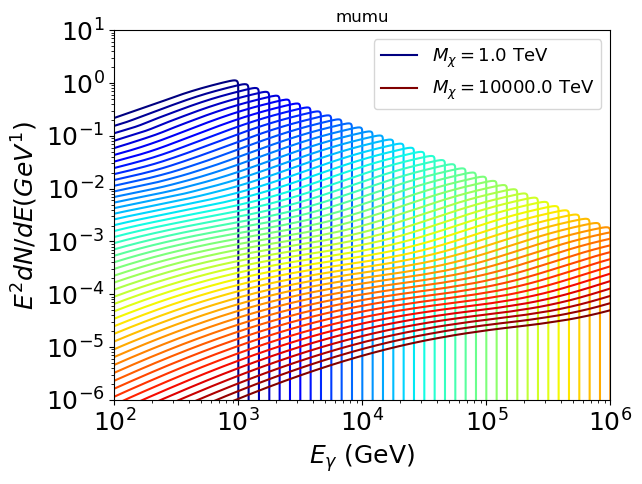
\includegraphics[scale=0.27]{figures/mtd_hawc_dm/hdm_mumu.png} &
        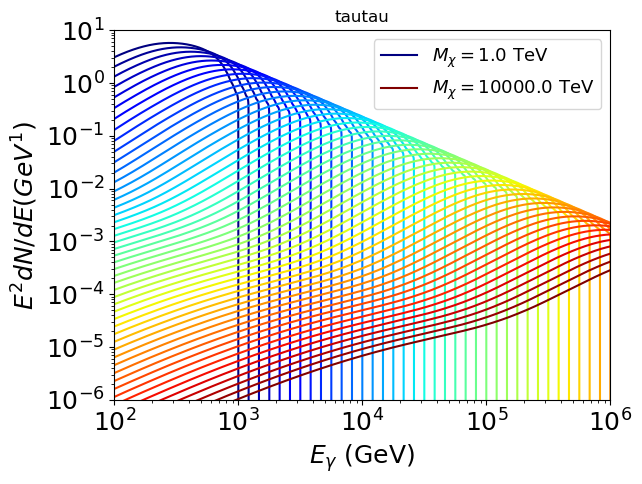
\includegraphics[scale=0.27]{figures/mtd_hawc_dm/hdm_tautau.png} &
        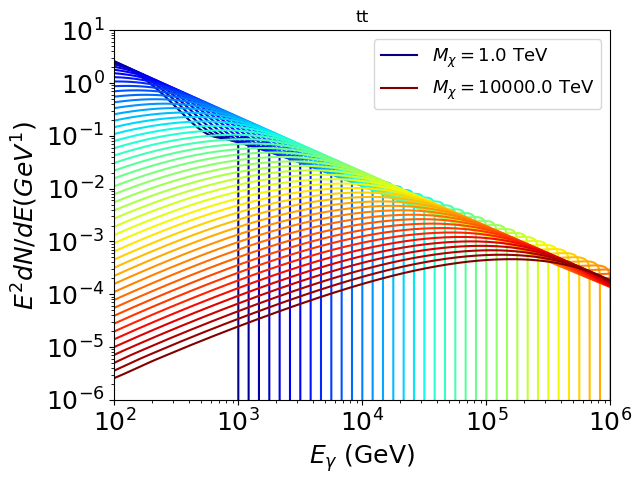
\includegraphics[scale=0.27]{figures/mtd_hawc_dm/hdm_tt.png} \\
        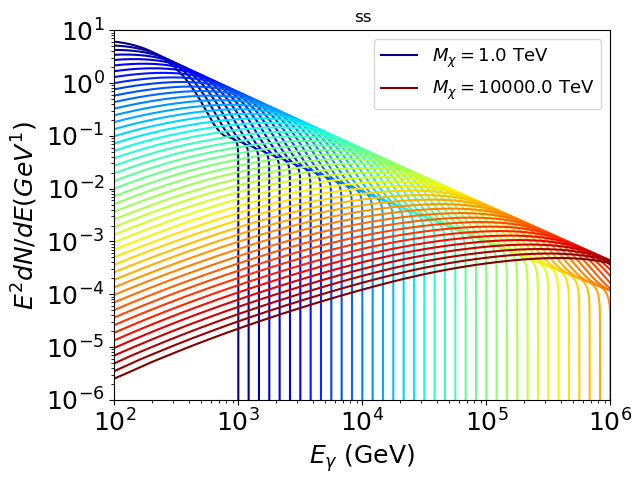
\includegraphics[scale=0.27]{figures/mtd_hawc_dm/hdm_ss.png} &
        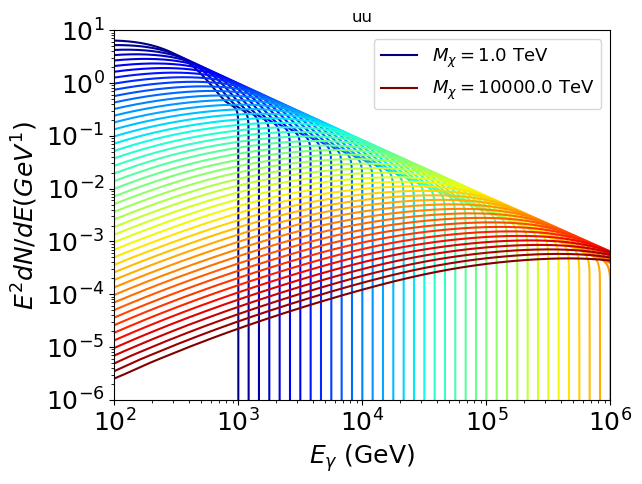
\includegraphics[scale=0.27]{figures/mtd_hawc_dm/hdm_uu.png} &
        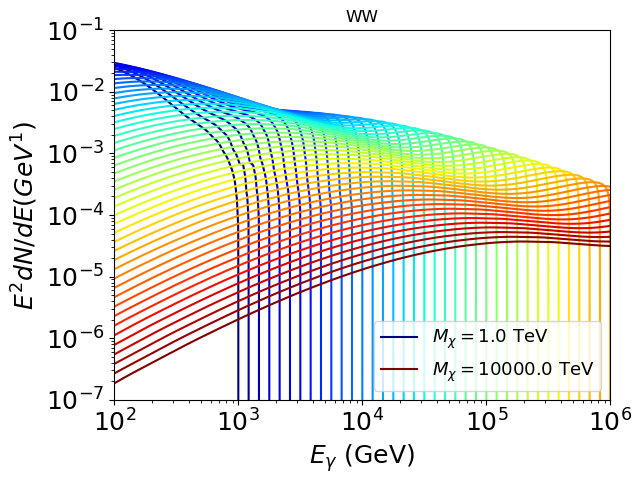
\includegraphics[scale=0.27]{figures/mtd_hawc_dm/hdm_ww.png} \\
        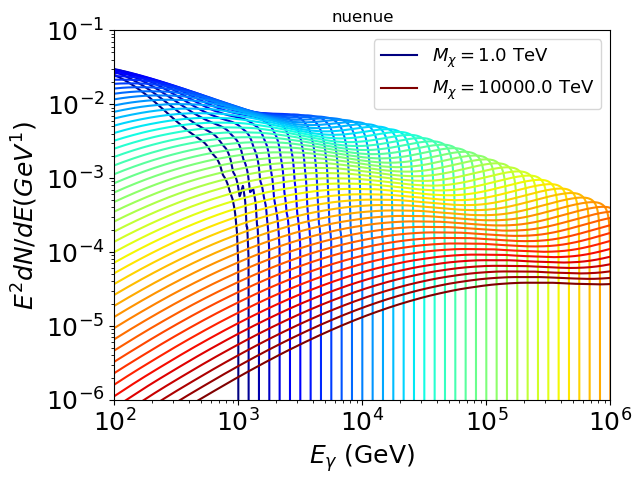
\includegraphics[scale=0.27]{figures/mtd_hawc_dm/hdm_nuenue.png} &
        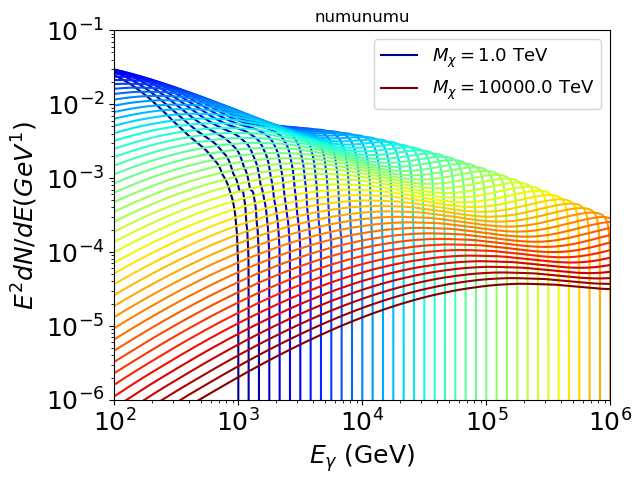
\includegraphics[scale=0.27]{figures/mtd_hawc_dm/hdm_numunumu.png} &
        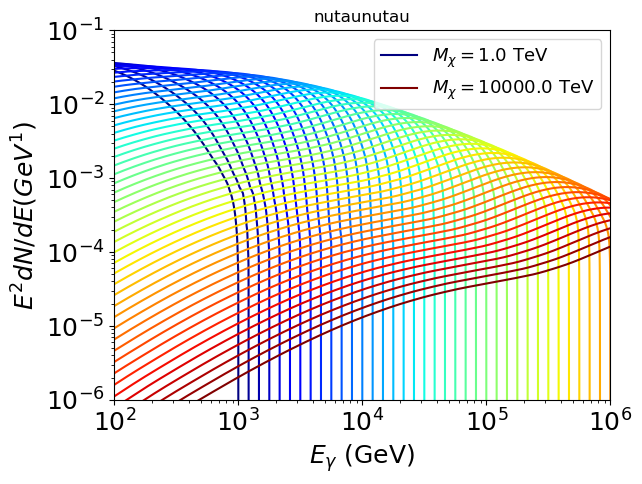
\includegraphics[scale=0.27]{figures/mtd_hawc_dm/hdm_nutaunutau.png} \\
    \end{tabular}
    }\caption{Sister figure to \Cref{fig:hdm_gamma_lines} for remaining SM primary annihilation channels studied for this thesis. These did not require any post generation smoothing and so are directly pulled from \cite{HDMSpectra} with a binning scheme most helpful for a HAWC analysis.
    }\label{fig:apdx_mtd_spectra}
\end{figure}